% A gorilla made with TikZ shapes. Use: % A gorilla made with TikZ shapes. Use: % A gorilla made with TikZ shapes. Use: % A gorilla made with TikZ shapes. Use: \input{gorilla} (needs \usepackage{tikz}).
% Change the size with \newcommand{\gorillascale}{0.8} before \input.
\providecommand{\gorillascale}{1}
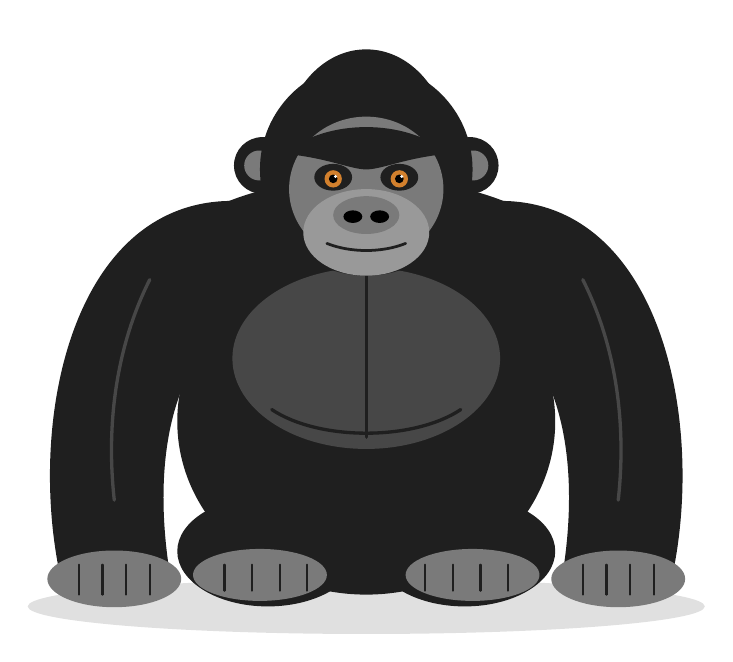
\begin{tikzpicture}[scale=\gorillascale, line cap=round, line join=round]
  \colorlet{fur}{black!88}
  \colorlet{furlight}{black!72}
  \colorlet{skin}{black!52}
  \colorlet{skinlight}{black!40}

  % ground shadow
  \fill[black!12] (0,-3.25) ellipse [x radius=4.3, y radius=0.35];

  % shoulders and body
  \fill[fur] (0,0.7) ellipse [x radius=2.9, y radius=1.5];
  \fill[fur] (0,-0.9) ellipse [x radius=2.4, y radius=2.2];

  % chest
  \fill[furlight] (0,-0.1) ellipse [x radius=1.7, y radius=1.15];
  \draw[fur, line width=1.2pt] (0,0.95) -- (0,-1.1);
  \draw[fur, line width=1.2pt] (-1.2,-0.75) .. controls (-0.6,-1.15) and (0.6,-1.15) .. (1.2,-0.75);

  % feet
  \foreach \s in {-1,1} {
    \begin{scope}[xscale=\s]
      \fill[fur] (1.25,-2.55) ellipse [x radius=1.15, y radius=0.7];
      \fill[skin] (1.35,-2.85) ellipse [x radius=0.85, y radius=0.33];
      \foreach \t in {0.75,1.1,1.45,1.8}
        \draw[fur, line width=0.8pt] (\t,-2.72) -- (\t,-3.05);
    \end{scope}
  }

  % arms and fists
  \foreach \s in {-1,1} {
    \begin{scope}[xscale=\s]
      \fill[fur] (1.7,1.9)
        .. controls (3.7,1.9) and (4.3,-0.8) .. (3.9,-2.8)
        -- (2.5,-2.8)
        .. controls (2.7,-1.5) and (2.5,-0.4) .. (1.9,0.2) -- cycle;
      \draw[furlight, line width=1.2pt] (2.75,0.9) .. controls (3.2,0.0) and (3.3,-1.0) .. (3.2,-1.9);
      \fill[skin] (3.2,-2.9) ellipse [x radius=0.85, y radius=0.36];
      \foreach \t in {2.75,3.05,3.35,3.65}
        \draw[fur, line width=0.8pt] (\t,-2.72) -- (\t,-3.1);
    \end{scope}
  }

  % head: ears, skull, crest
  \foreach \s in {-1,1} {
    \fill[fur] (\s*1.32,2.35) circle [radius=0.36];
    \fill[skin] (\s*1.36,2.35) circle [radius=0.19];
  }
  \fill[fur] (0,2.3) ellipse [x radius=1.35, y radius=1.35];
  \fill[fur] (-1.0,3.0) .. controls (-0.6,4.1) and (0.6,4.1) .. (1.0,3.0) -- cycle;

  % face
  \fill[skin] (0,2.05) ellipse [x radius=0.98, y radius=0.92];
  \fill[skinlight] (0,1.5) ellipse [x radius=0.8, y radius=0.55];

  % brow
  \fill[fur] (-1.05,2.5) .. controls (-0.5,2.95) and (0.5,2.95) .. (1.05,2.5)
    .. controls (0.5,2.45) and (0.2,2.3) .. (0,2.3)
    .. controls (-0.2,2.3) and (-0.5,2.45) .. cycle;

  % eyes
  \foreach \s in {-1,1} {
    \fill[fur] (\s*0.42,2.2) ellipse [x radius=0.24, y radius=0.17];
    \fill[brown!70!orange] (\s*0.42,2.18) circle [radius=0.11];
    \fill[black] (\s*0.42,2.18) circle [radius=0.055];
    \fill[white] (\s*0.42+0.03,2.21) circle [radius=0.02];
  }

  % nose and mouth
  \fill[skin] (0,1.72) ellipse [x radius=0.42, y radius=0.24];
  \foreach \s in {-1,1}
    \fill[black] (\s*0.17,1.7) ellipse [x radius=0.12, y radius=0.08];
  \draw[fur, line width=1pt] (-0.5,1.36) .. controls (-0.2,1.24) and (0.2,1.24) .. (0.5,1.36);
\end{tikzpicture}
 (needs \usepackage{tikz}).
% Change the size with \newcommand{\gorillascale}{0.8} before \input.
\providecommand{\gorillascale}{1}
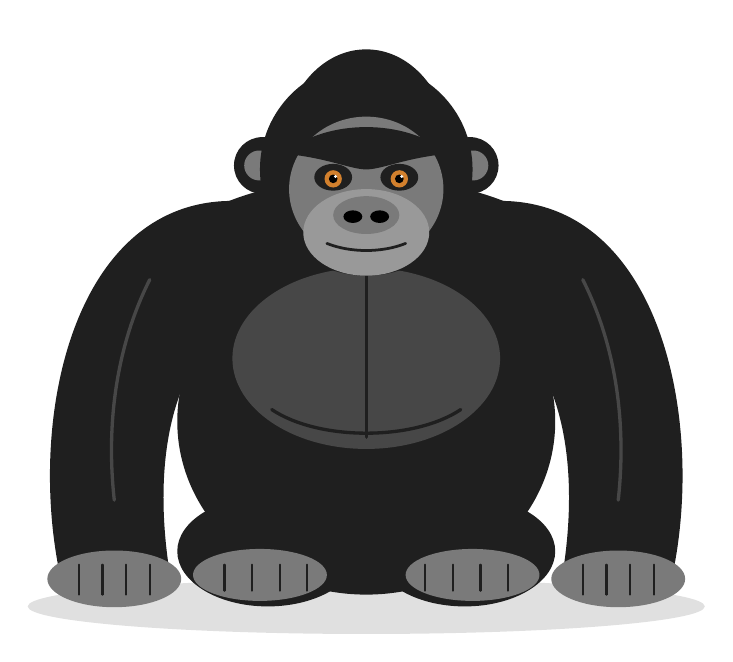
\begin{tikzpicture}[scale=\gorillascale, line cap=round, line join=round]
  \colorlet{fur}{black!88}
  \colorlet{furlight}{black!72}
  \colorlet{skin}{black!52}
  \colorlet{skinlight}{black!40}

  % ground shadow
  \fill[black!12] (0,-3.25) ellipse [x radius=4.3, y radius=0.35];

  % shoulders and body
  \fill[fur] (0,0.7) ellipse [x radius=2.9, y radius=1.5];
  \fill[fur] (0,-0.9) ellipse [x radius=2.4, y radius=2.2];

  % chest
  \fill[furlight] (0,-0.1) ellipse [x radius=1.7, y radius=1.15];
  \draw[fur, line width=1.2pt] (0,0.95) -- (0,-1.1);
  \draw[fur, line width=1.2pt] (-1.2,-0.75) .. controls (-0.6,-1.15) and (0.6,-1.15) .. (1.2,-0.75);

  % feet
  \foreach \s in {-1,1} {
    \begin{scope}[xscale=\s]
      \fill[fur] (1.25,-2.55) ellipse [x radius=1.15, y radius=0.7];
      \fill[skin] (1.35,-2.85) ellipse [x radius=0.85, y radius=0.33];
      \foreach \t in {0.75,1.1,1.45,1.8}
        \draw[fur, line width=0.8pt] (\t,-2.72) -- (\t,-3.05);
    \end{scope}
  }

  % arms and fists
  \foreach \s in {-1,1} {
    \begin{scope}[xscale=\s]
      \fill[fur] (1.7,1.9)
        .. controls (3.7,1.9) and (4.3,-0.8) .. (3.9,-2.8)
        -- (2.5,-2.8)
        .. controls (2.7,-1.5) and (2.5,-0.4) .. (1.9,0.2) -- cycle;
      \draw[furlight, line width=1.2pt] (2.75,0.9) .. controls (3.2,0.0) and (3.3,-1.0) .. (3.2,-1.9);
      \fill[skin] (3.2,-2.9) ellipse [x radius=0.85, y radius=0.36];
      \foreach \t in {2.75,3.05,3.35,3.65}
        \draw[fur, line width=0.8pt] (\t,-2.72) -- (\t,-3.1);
    \end{scope}
  }

  % head: ears, skull, crest
  \foreach \s in {-1,1} {
    \fill[fur] (\s*1.32,2.35) circle [radius=0.36];
    \fill[skin] (\s*1.36,2.35) circle [radius=0.19];
  }
  \fill[fur] (0,2.3) ellipse [x radius=1.35, y radius=1.35];
  \fill[fur] (-1.0,3.0) .. controls (-0.6,4.1) and (0.6,4.1) .. (1.0,3.0) -- cycle;

  % face
  \fill[skin] (0,2.05) ellipse [x radius=0.98, y radius=0.92];
  \fill[skinlight] (0,1.5) ellipse [x radius=0.8, y radius=0.55];

  % brow
  \fill[fur] (-1.05,2.5) .. controls (-0.5,2.95) and (0.5,2.95) .. (1.05,2.5)
    .. controls (0.5,2.45) and (0.2,2.3) .. (0,2.3)
    .. controls (-0.2,2.3) and (-0.5,2.45) .. cycle;

  % eyes
  \foreach \s in {-1,1} {
    \fill[fur] (\s*0.42,2.2) ellipse [x radius=0.24, y radius=0.17];
    \fill[brown!70!orange] (\s*0.42,2.18) circle [radius=0.11];
    \fill[black] (\s*0.42,2.18) circle [radius=0.055];
    \fill[white] (\s*0.42+0.03,2.21) circle [radius=0.02];
  }

  % nose and mouth
  \fill[skin] (0,1.72) ellipse [x radius=0.42, y radius=0.24];
  \foreach \s in {-1,1}
    \fill[black] (\s*0.17,1.7) ellipse [x radius=0.12, y radius=0.08];
  \draw[fur, line width=1pt] (-0.5,1.36) .. controls (-0.2,1.24) and (0.2,1.24) .. (0.5,1.36);
\end{tikzpicture}
 (needs \usepackage{tikz}).
% Change the size with \newcommand{\gorillascale}{0.8} before \input.
\providecommand{\gorillascale}{1}
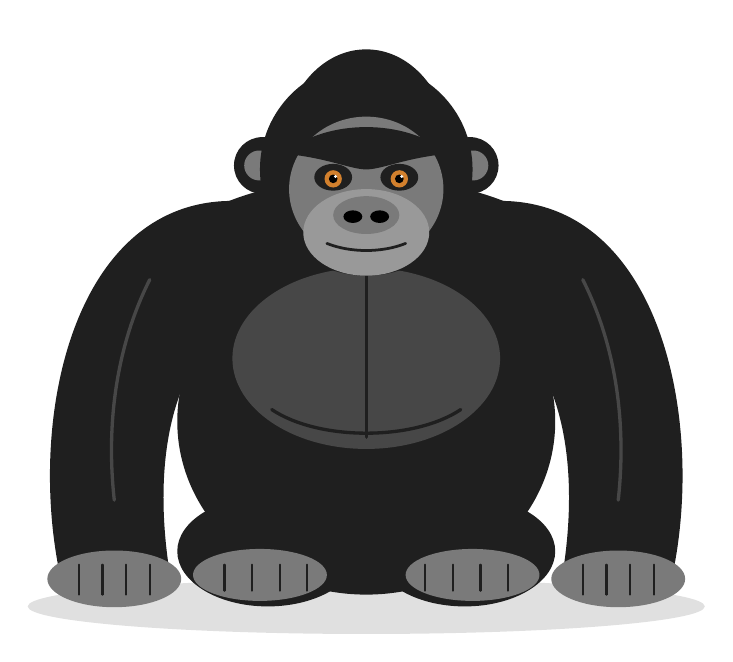
\begin{tikzpicture}[scale=\gorillascale, line cap=round, line join=round]
  \colorlet{fur}{black!88}
  \colorlet{furlight}{black!72}
  \colorlet{skin}{black!52}
  \colorlet{skinlight}{black!40}

  % ground shadow
  \fill[black!12] (0,-3.25) ellipse [x radius=4.3, y radius=0.35];

  % shoulders and body
  \fill[fur] (0,0.7) ellipse [x radius=2.9, y radius=1.5];
  \fill[fur] (0,-0.9) ellipse [x radius=2.4, y radius=2.2];

  % chest
  \fill[furlight] (0,-0.1) ellipse [x radius=1.7, y radius=1.15];
  \draw[fur, line width=1.2pt] (0,0.95) -- (0,-1.1);
  \draw[fur, line width=1.2pt] (-1.2,-0.75) .. controls (-0.6,-1.15) and (0.6,-1.15) .. (1.2,-0.75);

  % feet
  \foreach \s in {-1,1} {
    \begin{scope}[xscale=\s]
      \fill[fur] (1.25,-2.55) ellipse [x radius=1.15, y radius=0.7];
      \fill[skin] (1.35,-2.85) ellipse [x radius=0.85, y radius=0.33];
      \foreach \t in {0.75,1.1,1.45,1.8}
        \draw[fur, line width=0.8pt] (\t,-2.72) -- (\t,-3.05);
    \end{scope}
  }

  % arms and fists
  \foreach \s in {-1,1} {
    \begin{scope}[xscale=\s]
      \fill[fur] (1.7,1.9)
        .. controls (3.7,1.9) and (4.3,-0.8) .. (3.9,-2.8)
        -- (2.5,-2.8)
        .. controls (2.7,-1.5) and (2.5,-0.4) .. (1.9,0.2) -- cycle;
      \draw[furlight, line width=1.2pt] (2.75,0.9) .. controls (3.2,0.0) and (3.3,-1.0) .. (3.2,-1.9);
      \fill[skin] (3.2,-2.9) ellipse [x radius=0.85, y radius=0.36];
      \foreach \t in {2.75,3.05,3.35,3.65}
        \draw[fur, line width=0.8pt] (\t,-2.72) -- (\t,-3.1);
    \end{scope}
  }

  % head: ears, skull, crest
  \foreach \s in {-1,1} {
    \fill[fur] (\s*1.32,2.35) circle [radius=0.36];
    \fill[skin] (\s*1.36,2.35) circle [radius=0.19];
  }
  \fill[fur] (0,2.3) ellipse [x radius=1.35, y radius=1.35];
  \fill[fur] (-1.0,3.0) .. controls (-0.6,4.1) and (0.6,4.1) .. (1.0,3.0) -- cycle;

  % face
  \fill[skin] (0,2.05) ellipse [x radius=0.98, y radius=0.92];
  \fill[skinlight] (0,1.5) ellipse [x radius=0.8, y radius=0.55];

  % brow
  \fill[fur] (-1.05,2.5) .. controls (-0.5,2.95) and (0.5,2.95) .. (1.05,2.5)
    .. controls (0.5,2.45) and (0.2,2.3) .. (0,2.3)
    .. controls (-0.2,2.3) and (-0.5,2.45) .. cycle;

  % eyes
  \foreach \s in {-1,1} {
    \fill[fur] (\s*0.42,2.2) ellipse [x radius=0.24, y radius=0.17];
    \fill[brown!70!orange] (\s*0.42,2.18) circle [radius=0.11];
    \fill[black] (\s*0.42,2.18) circle [radius=0.055];
    \fill[white] (\s*0.42+0.03,2.21) circle [radius=0.02];
  }

  % nose and mouth
  \fill[skin] (0,1.72) ellipse [x radius=0.42, y radius=0.24];
  \foreach \s in {-1,1}
    \fill[black] (\s*0.17,1.7) ellipse [x radius=0.12, y radius=0.08];
  \draw[fur, line width=1pt] (-0.5,1.36) .. controls (-0.2,1.24) and (0.2,1.24) .. (0.5,1.36);
\end{tikzpicture}
 (needs \usepackage{tikz}).
% Change the size with \newcommand{\gorillascale}{0.8} before \input.
\providecommand{\gorillascale}{1}
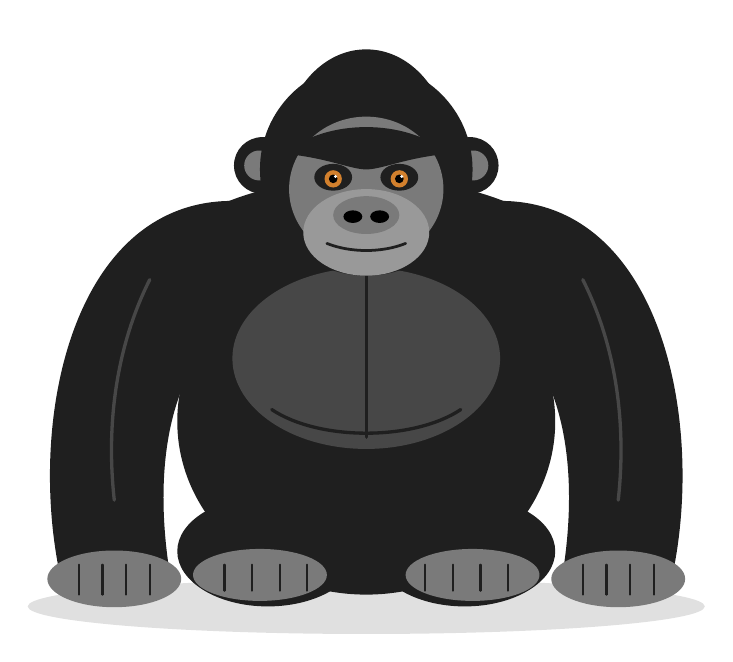
\begin{tikzpicture}[scale=\gorillascale, line cap=round, line join=round]
  \colorlet{fur}{black!88}
  \colorlet{furlight}{black!72}
  \colorlet{skin}{black!52}
  \colorlet{skinlight}{black!40}

  % ground shadow
  \fill[black!12] (0,-3.25) ellipse [x radius=4.3, y radius=0.35];

  % shoulders and body
  \fill[fur] (0,0.7) ellipse [x radius=2.9, y radius=1.5];
  \fill[fur] (0,-0.9) ellipse [x radius=2.4, y radius=2.2];

  % chest
  \fill[furlight] (0,-0.1) ellipse [x radius=1.7, y radius=1.15];
  \draw[fur, line width=1.2pt] (0,0.95) -- (0,-1.1);
  \draw[fur, line width=1.2pt] (-1.2,-0.75) .. controls (-0.6,-1.15) and (0.6,-1.15) .. (1.2,-0.75);

  % feet
  \foreach \s in {-1,1} {
    \begin{scope}[xscale=\s]
      \fill[fur] (1.25,-2.55) ellipse [x radius=1.15, y radius=0.7];
      \fill[skin] (1.35,-2.85) ellipse [x radius=0.85, y radius=0.33];
      \foreach \t in {0.75,1.1,1.45,1.8}
        \draw[fur, line width=0.8pt] (\t,-2.72) -- (\t,-3.05);
    \end{scope}
  }

  % arms and fists
  \foreach \s in {-1,1} {
    \begin{scope}[xscale=\s]
      \fill[fur] (1.7,1.9)
        .. controls (3.7,1.9) and (4.3,-0.8) .. (3.9,-2.8)
        -- (2.5,-2.8)
        .. controls (2.7,-1.5) and (2.5,-0.4) .. (1.9,0.2) -- cycle;
      \draw[furlight, line width=1.2pt] (2.75,0.9) .. controls (3.2,0.0) and (3.3,-1.0) .. (3.2,-1.9);
      \fill[skin] (3.2,-2.9) ellipse [x radius=0.85, y radius=0.36];
      \foreach \t in {2.75,3.05,3.35,3.65}
        \draw[fur, line width=0.8pt] (\t,-2.72) -- (\t,-3.1);
    \end{scope}
  }

  % head: ears, skull, crest
  \foreach \s in {-1,1} {
    \fill[fur] (\s*1.32,2.35) circle [radius=0.36];
    \fill[skin] (\s*1.36,2.35) circle [radius=0.19];
  }
  \fill[fur] (0,2.3) ellipse [x radius=1.35, y radius=1.35];
  \fill[fur] (-1.0,3.0) .. controls (-0.6,4.1) and (0.6,4.1) .. (1.0,3.0) -- cycle;

  % face
  \fill[skin] (0,2.05) ellipse [x radius=0.98, y radius=0.92];
  \fill[skinlight] (0,1.5) ellipse [x radius=0.8, y radius=0.55];

  % brow
  \fill[fur] (-1.05,2.5) .. controls (-0.5,2.95) and (0.5,2.95) .. (1.05,2.5)
    .. controls (0.5,2.45) and (0.2,2.3) .. (0,2.3)
    .. controls (-0.2,2.3) and (-0.5,2.45) .. cycle;

  % eyes
  \foreach \s in {-1,1} {
    \fill[fur] (\s*0.42,2.2) ellipse [x radius=0.24, y radius=0.17];
    \fill[brown!70!orange] (\s*0.42,2.18) circle [radius=0.11];
    \fill[black] (\s*0.42,2.18) circle [radius=0.055];
    \fill[white] (\s*0.42+0.03,2.21) circle [radius=0.02];
  }

  % nose and mouth
  \fill[skin] (0,1.72) ellipse [x radius=0.42, y radius=0.24];
  \foreach \s in {-1,1}
    \fill[black] (\s*0.17,1.7) ellipse [x radius=0.12, y radius=0.08];
  \draw[fur, line width=1pt] (-0.5,1.36) .. controls (-0.2,1.24) and (0.2,1.24) .. (0.5,1.36);
\end{tikzpicture}
